\documentclass[
    convert={density=300,outext=.png}
]{standalone}
\usepackage{graphicx}

\usepackage{tikz}

\usetikzlibrary{arrows,decorations.pathreplacing,backgrounds,positioning,fit,petri}

\begin{document}
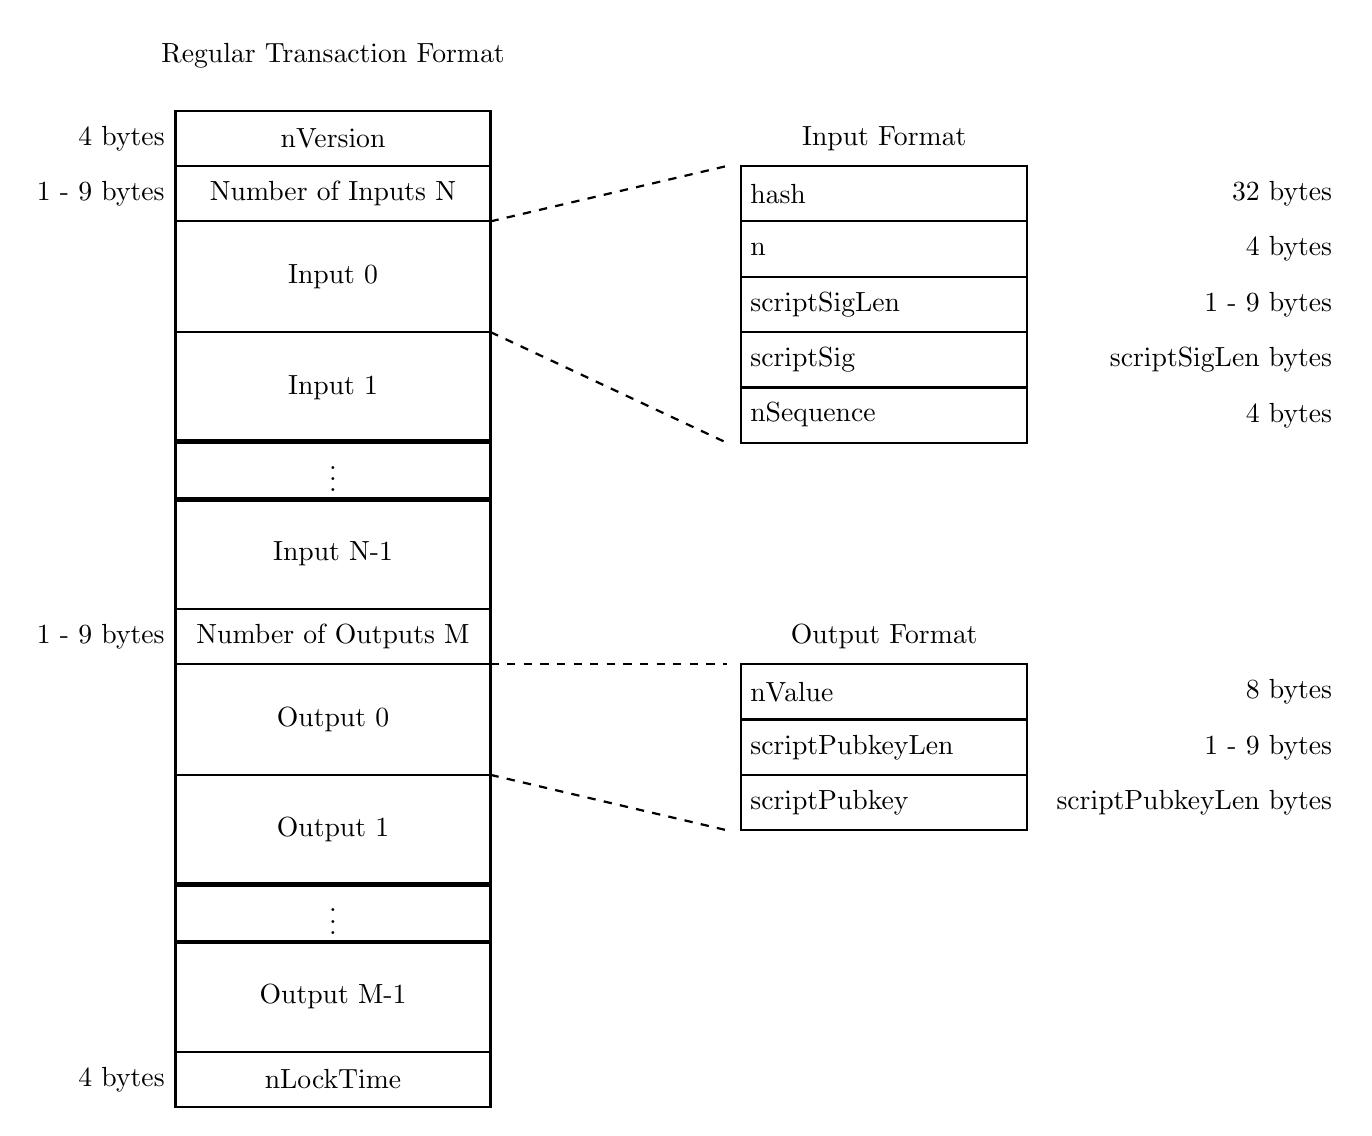
\begin{tikzpicture}
    [
        Field1/.style={rectangle,minimum width=4cm,minimum height=20pt,draw, thick, align=center},
        Field2/.style={rectangle,minimum width=4cm,minimum height=40pt,draw, thick, align=center},
        Field3/.style={rectangle,minimum width=3.6cm,minimum height=20pt,draw, thick, text width=3.4cm},
        TextBox1/.style={minimum width=4cm, minimum height=20pt, align=center},
        TextBox2/.style={minimum width=4cm, minimum height=20pt, text width=3.7cm, align=right}
    ]

    \node[TextBox1] (regular_transaction_format) at (2,380pt) {Regular Transaction Format};
    \node[Field1,label=left:4 bytes] (nVersion) at (2,350pt) {nVersion};
    \node[Field1,label=left:1 - 9 bytes] (Number_of_Inputs_N) at (2,330pt) {Number of Inputs N};
    \node[Field2] (Input0) at (2,300pt) {Input 0};
    \node[Field2] (Input1) at (2,260pt) {Input 1};
    \node[Field1] (InputEllipsis) at (2,230pt) {\vdots};
    \node[Field2] (InputN-1) at (2,200pt) {Input N-1};
    \node[Field1,label=left:1 - 9 bytes] (Number_of_Outputs_M) at (2,170pt) {Number of Outputs M};
    \node[Field2] (Output0) at (2,140pt) {Output 0};
    \node[Field2] (Output1) at (2,100pt) {Output 1};
    \node[Field1] (OutputEllipsis) at (2,70pt) {$\vdots$};
    \node[Field2] (OutputM-1) at (2,40pt) {Output M-1};
    \node[Field1,label=left:4 bytes] (nLockTime) at (2,10pt) {nLockTime};

    \node[TextBox1] (input_format) at (9,350pt) {Input Format};
    \node[Field3] (hash) at (9,330pt) {hash};
    \node[TextBox2,right=0pt of hash] (sizeof_hash) {32 bytes};
    \node[Field3] (n) at (9,310pt) {n};
    \node[TextBox2,right=0pt of n] (sizeof_n) {4 bytes};
    \node[Field3] (scriptSigLen) at (9,290pt) {scriptSigLen};
    \node[TextBox2,right=0pt of scriptSigLen] (sizeof_scriptSigLen) {1 - 9 bytes};
    \node[Field3] (scriptSig) at (9,270pt) {scriptSig};
    \node[TextBox2,right=0pt of scriptSig] (sizeof_scriptSig) {scriptSigLen bytes};
    \node[Field3] (nSequence) at (9,250pt) {nSequence};
    \node[TextBox2,right=0pt of nSequence] (sizeof_nSequence) {4 bytes};

    \node[TextBox1] (output_format) at (9,170pt) {Output Format};
    \node[Field3] (nValue) at (9,150pt) {nValue};
    \node[TextBox2,right=0pt of nValue] (sizeof_nValue) {8 bytes};
    \node[Field3] (scriptPubkeyLen) at (9,130pt) {scriptPubkeyLen};
    \node[TextBox2,right=0pt of scriptPubkeyLen] (sizeof_scriptPubkeyLen) {1 - 9 bytes};
    \node[Field3] (scriptPubkey) at (9,110pt) {scriptPubkey};
    \node[TextBox2,right=0pt of scriptPubkey] (sizeof_scriptPubkey) {scriptPubkeyLen bytes};

    \draw[dashed, thick] (4cm, 320pt) -- (7cm, 340pt);
    \draw[dashed, thick] (4cm, 280pt) -- (7cm, 240pt);
    \draw[dashed, thick] (4cm, 160pt) -- (7cm, 160pt);
    \draw[dashed, thick] (4cm, 120pt) -- (7cm, 100pt);
\end{tikzpicture}
\end{document}